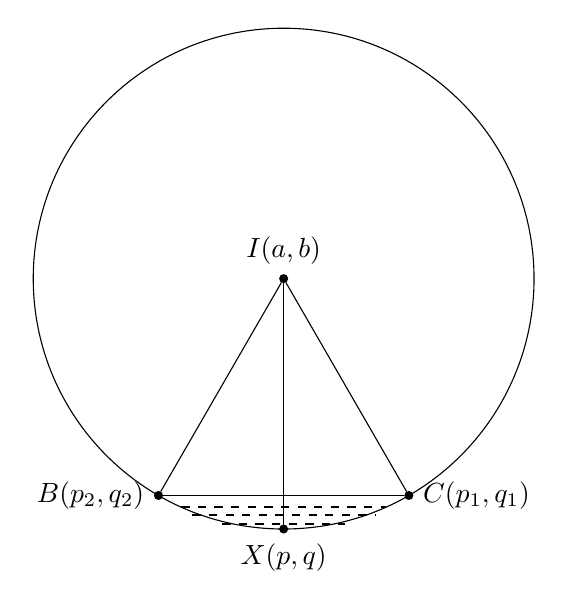
\begin{tikzpicture}
[
scale =2,
>=stealth,
point/.style = {draw, circle, fill = black, inner sep = 1pt},
]

\def\rad{1.59}
\coordinate [point, label={above : $I{(a,b)}$ }] (I) at (0, 0);
\draw (I) circle (\rad);

\node (C) at (300:{\rad})[point,label = right:$C{(p_1,q_1)}$] {};

\node (X) at (270:{\rad}) [point,label = below:$X{(p,q)}$] {};

\node (B) at (240:{\rad}) [point,label = left:$B{(p_2,q_2)}$] {};

\draw (C) -- (I);
\draw (B) -- (I);
\draw (B) -- (C);
\draw (I) -- (X);

\draw[black,thick,dashed](-0.65,-1.45) -- (0.65,-1.45);
\draw[black,thick,dashed](-0.58,-1.5) -- (0.58,-1.5);
\draw[black,thick,dashed](-0.39,-1.56) -- (0.39,-1.56);
\end{tikzpicture}
